\section{Network scans}
\paragraph{ICMP scans} The most simple scanning technique is sending \texttt{ICMP} requests and waiting for a possible \texttt{ICMP echo reply}. Network administrators often configure host to ignore \texttt{ICMP packets}.

\paragraph{TCP port scanning}

Three common TCP port scanning techniques are:

\begin{itemize}
    \item \textbf{TCP Connect Scan (Full Handshake)}: perform a complete TCP handshake (\texttt{SYN}, \texttt{SYN+ACK}, \texttt{ACK}) as shown in Figure~\ref{fig:tcp1}. This technique is easy to implement since it relies on the operating system's normal socket API, but it is slower and establishes a real TCP connection.
    
    \begin{itemize}
        \item \texttt{SYN+ACK} received $\rightarrow$ port \textbf{open}.
        \item \texttt{RST} received $\rightarrow$ port \textbf{closed}.
        \item No response $\rightarrow$ port \textbf{filtered} or target unreachable.
    \end{itemize}

    \item \textbf{TCP SYN Scan (Half-Open Scan)}: send a \texttt{SYN} packet and, if a \texttt{SYN+ACK} is received, immediately reply with a \texttt{RST} instead of completing the handshake (Figure~\ref{fig:tcp2}). Since no connection is established, this technique is faster and more discreet.
    
    \begin{itemize}
        \item \texttt{SYN+ACK} received $\rightarrow$ port \textbf{open}.
        \item \texttt{RST} received $\rightarrow$ port \textbf{closed}.
        \item No response $\rightarrow$ port \textbf{filtered} or target unreachable.
    \end{itemize}

    \item \textbf{TCP Xmas-Tree Scan}: send a packet with the \texttt{FIN}, \texttt{PSH} and \texttt{URG} flags set. According to RFC-compliant TCP implementations, a closed port should respond with a \texttt{RST}, while an open port should ignore the packet.
    
    \begin{itemize}
        \item \texttt{RST} received $\rightarrow$ port \textbf{closed}.
        \item No response $\rightarrow$ port \textbf{open or filtered}.
    \end{itemize}
\end{itemize}


\begin{figure}
    \centering
    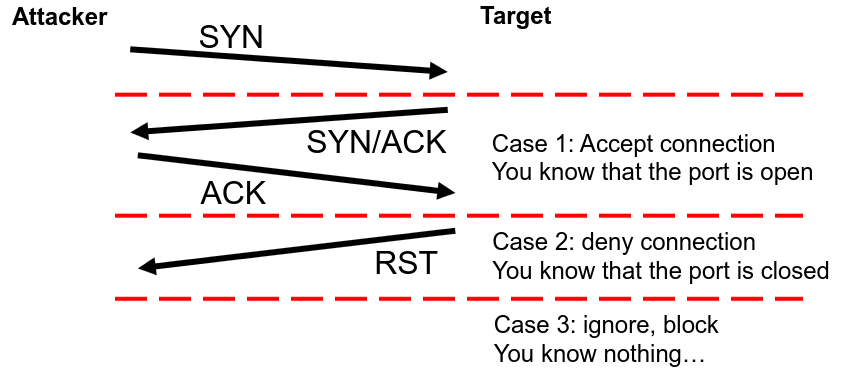
\includegraphics[width=0.7\linewidth]{Figures/TCP_Scan_1.png}
    \caption{Full TCP Scan}
    \label{fig:tcp1}
\end{figure}

\begin{figure}
    \centering
    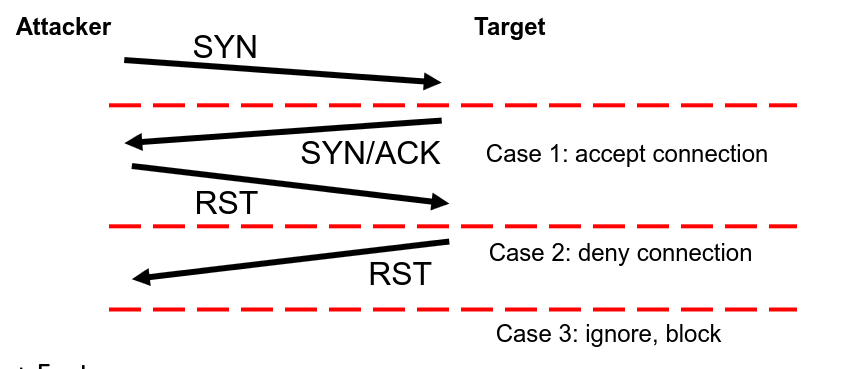
\includegraphics[width=0.7\linewidth]{Figures/TCP_Scan_2.png}
    \caption{Half TCP Scan}
    \label{fig:tcp2}
\end{figure}

\paragraph{UDP Scan}

UDP scanning is more difficult than TCP scanning because UDP is a \textbf{connectionless} protocol.

Two common approaches are:

\begin{itemize}
    \item \textbf{Negative-response scanning}: send a UDP packet and wait for an ICMP \texttt{Port Unreachable} message. Receiving such a message indicates that the port is \textbf{closed}. If no response is received, the port may be open, filtered, or the ICMP message may have been blocked.

    \item \textbf{Positive-response scanning}: send a valid request for the expected service (e.g., a DNS query on port 53) and wait for a response. Receiving a valid response indicates that the port is \textbf{open}. If no response is received, no reliable conclusion can be drawn.
\end{itemize}

UDP scans are therefore less reliable than TCP scans since many UDP services do not respond to invalid requests and ICMP messages may be filtered by firewalls.

\paragraph{Application Layer Scan} it is possible as well for example to scan many \texttt{URL's} to see which web application is running on a server 